% !TEX TS-program = pdflatexmk

%%%%%%%%%%%%%%%%%%%%%%%%%%%%%%%%%%%%%%%%%%%%%%%%%%%%%%%%%%%%%%%%%%
%%%%%%%% ICML 2016 EXAMPLE LATEX SUBMISSION FILE %%%%%%%%%%%%%%%%%
%%%%%%%%%%%%%%%%%%%%%%%%%%%%%%%%%%%%%%%%%%%%%%%%%%%%%%%%%%%%%%%%%%

% Use the following line _only_ if you're still using LaTeX 2.09.
%\documentstyle[icml2016,epsf,natbib]{article}
% If you rely on Latex2e packages, like most moden people use this:
\documentclass{article}

% use Times
\usepackage{times}
% For figures
\usepackage{graphicx} % more modern
%\usepackage{epsfig} % less modern
\usepackage{subfigure}

% For citations
\usepackage{natbib}

% For algorithms
\usepackage{algorithm}
\usepackage{algorithmic}

% As of 2011, we use the hyperref package to produce hyperlinks in the
% resulting PDF.  If this breaks your system, please commend out the
% following usepackage line and replace \usepackage{icml2016} with
% \usepackage[nohyperref]{icml2016} above.
\usepackage{hyperref}

% Packages hyperref and algorithmic misbehave sometimes.  We can fix
% this with the following command.
\newcommand{\theHalgorithm}{\arabic{algorithm}}

% Employ the following version of the ``usepackage'' statement for
% submitting the draft version of the paper for review.  This will set
% the note in the first column to ``Under review.  Do not distribute.''
\usepackage{icml2016}

% Employ this version of the ``usepackage'' statement after the paper has
% been accepted, when creating the final version.  This will set the
% note in the first column to ``Proceedings of the...''
%\usepackage[accepted]{icml2016}


\usepackage{amsthm}
\usepackage{amssymb}
\usepackage{amsmath}

% The \icmltitle you define below is probably too long as a header.
% Therefore, a short form for the running title is supplied here:
\icmltitlerunning{Particle Thompson Sampling for Knowledge Base Completion}

\begin{document}

\twocolumn[
\icmltitle{Particle Thompson Sampling for Knowledge Base Completion}

% It is OKAY to include author information, even for blind
% submissions: the style file will automatically remove it for you
% unless you've provided the [accepted] option to the icml2016
% package.
\icmlauthor{Your Name}{email@yourdomain.edu}
\icmladdress{Your Fantastic Institute,
            314159 Pi St., Palo Alto, CA 94306 USA}
\icmlauthor{Your CoAuthor's Name}{email@coauthordomain.edu}
\icmladdress{Their Fantastic Institute,
            27182 Exp St., Toronto, ON M6H 2T1 CANADA}

% You may provide any keywords that you
% find helpful for describing your paper; these are used to populate
% the "keywords" metadata in the PDF but will not be shown in the document
\icmlkeywords{machine learning, ICML}

\vskip 0.3in
]

\begin{abstract}
%Abstracts should be a single paragraph, between 4--6 sentences long, ideally.  Gross violations will trigger corrections at the camera-ready phase.
\end{abstract}

\section{Introduction}
Goal of this paper 1: Populating knowledge graph with an active label acquisition process corresponding to [B,C,A] in Figure \ref{fig:related3d}.

[B,C,P] could be an alternative direction (or both).

\section{Related Work}

\begin{figure}[t]
	\centering
	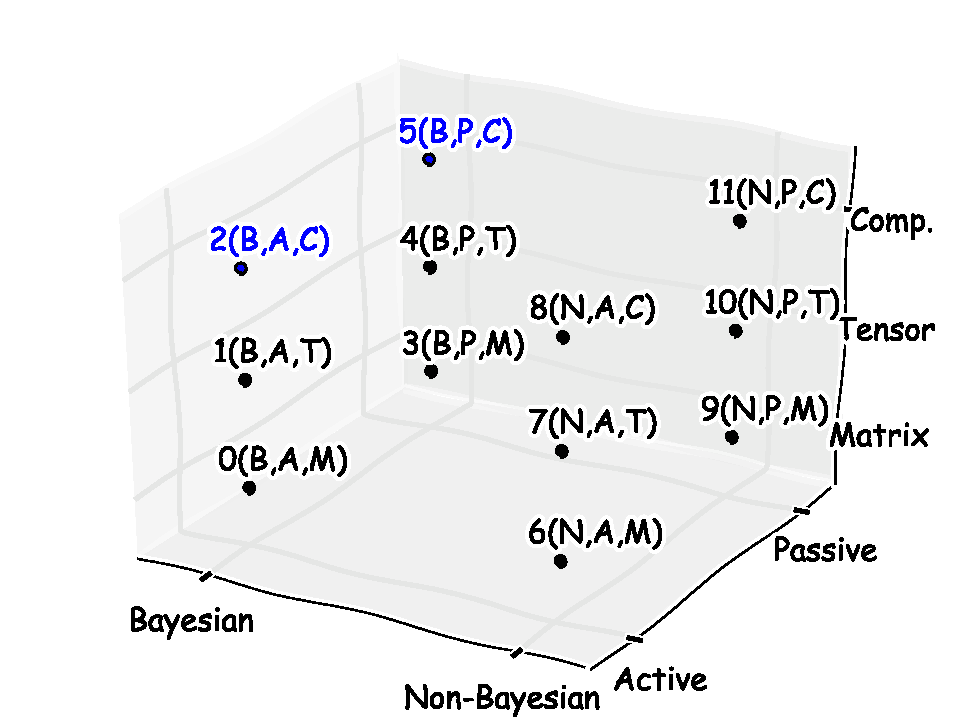
\includegraphics[width=\linewidth]{images/3d_plot.pdf}			
	\caption{\label{fig:related3d}Scope of our work}
\end{figure}

\begin{itemize}
\item [B,A,M] Efficient Thompson Sampling for OnlineMatrix-Factorization Recommendation\cite{kawale2015efficient}. Active learning and search on low-rank matrices \cite{sutherland2013active}.
\item [N,A,M] Matrix completion with queries \cite{ruchansky2015matrix}.
\item [B, P, M] PMF \cite{mnih2007probabilistic} ...
\item [N, P, M] NMF\cite{lee1999learning} ...
\item [B,T,A] ??
\item [B,T,P] Bayesian Tensor Factorisation models. CANDECOMP/PARAFAC (CP) decomposition \cite{xiong2010temporal,schmidt2009probabilistic}, CP and TUCKER3 \cite{yilmaz2012algorithms}
\item [N,T,A] Populating knowledge graph with active learning (IBM) \cite{kajino2015active}
\item [N,T,P] Rescal \cite{nickel2011three}, TransE \cite{bordes2013translating}, and many others.
\item [N,C,P] Compositional vector space model \cite{Neelakantan2015}, 
\end{itemize}

Might be relevant, but not positioned in the figure.
\begin{itemize}
\item Clustering based Bayesian approach for learning relations: Infinite relational model based on entity clustering \cite{kemp2006learning}.
\item Path ranking algorithm (graph feature model) \cite{Lao2010}
\end{itemize}

\section{Bayesian RESCAL}

For each entity $i$, $e_i \in \mathbb{R}^{D}$ is drawn from multivariate-normal distribution. Let $E$ be a $I \times D$ matrix representation of entities.
\begin{align}
\label{eqn:entity_gen}
e_i \sim {N}(\mathbf{0}, \sigma_e^2{I}_D)
\end{align}
For each relation $k$, we draw matrix $R_k \in \mathbb{R}^{D\times D}$ from zero-mean matrix normal distribution.
\begin{align}
\label{eqn:relation_gen}
R_k \sim \mathcal{N}_{D \times D}(\mathbf{0}, \sigma_r{I}_D, \sigma_r{I}_D) \\
\text{vec}(R_k) = r_k \sim N(\mathbf{0}, \sigma_r^2 I_{D^2})
\end{align}
For each triple $(i,k,j)$, we draw $x_{ikj}$
\begin{align}
\label{eqn:triple_gen}
x_{ikj} |e_i, e_j, R_k &\sim \mathcal{MN}(e_i^{\top} R_k e_j, \sigma_x^2)\\
& = \mathcal{N}(r_k^{\top} e_i \otimes e_j, \sigma_x^2)
\end{align}


\begin{figure}[t]
	\centering
	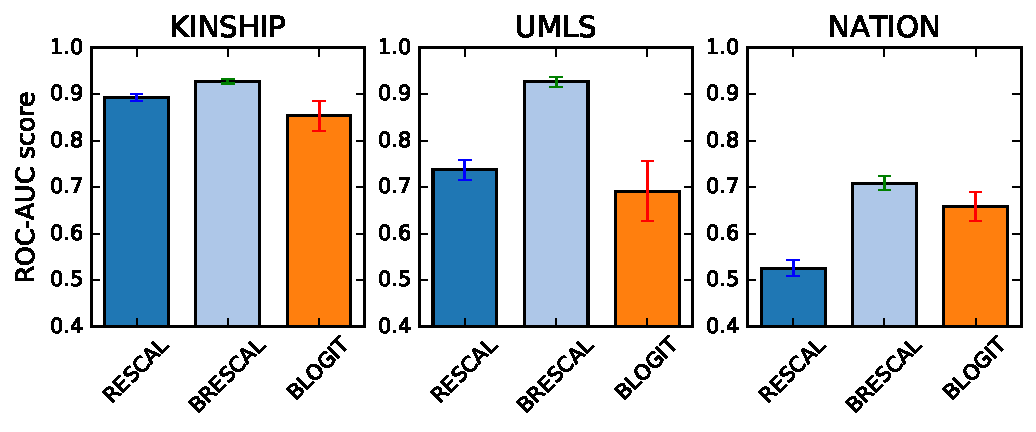
\includegraphics[width=\linewidth]{images/rescal_vs_brescal.pdf}			
	\caption{\label{fig:r_vs_br} ROC-AUC scores on three different datasets. BRESCAL and BLOGIT represent Bayesian RESCAL and Bayesian RESCAL with logistic regression outputs, respectively. BRESCAL consistently outperforms RESCAL across all datasets.}
\end{figure}


%For binary valued triples (Logistic regression):
%\begin{align}
%p(x_{ikj}=1) = \sigma(e_i^{\top} R_k e_j, \sigma_x^2)
%\end{align}

\section{Particle Thompson Sampling}
Let $\mathcal{X}^{t}$ be a set of observed triples up to time $t$.

The conditional distribution of $e_i$ given $\mathcal{R}$ and other entities $E_{-i}$
\begin{align} \label{eqn:sample_e}
p(e_i |E_{-i}, \mathcal{R}, \mathcal{X}^{t}, \sigma_e, \sigma_x) &= \mathcal{N}(e_i | \mu_i, \Lambda_i^{-1}),
\end{align}
where
\begin{align*}
\mu_i &= \frac{1}{\sigma_x^2}\Lambda_i^{-1}\xi_i \\
\Lambda_i &= \frac{1}{\sigma_x^2} \sum_{jk : x_{ikj} \in \mathcal{X}^{t}} (R_k e_j)(R_k e_j)^\top \\
&\quad+ \frac{1}{\sigma_x^2} \sum_{jk : x_{jki} \in \mathcal{X}^{t}} (R_k^\top e_j)(R_k^\top e_j)^\top+ \frac{1}{\sigma_e^2} {I}_D \\
\xi_i &= \sum_{jk : x_{ikj} \in \mathcal{X}^{t}}  x_{ikj} R_{k} e_{j} + \sum_{jk : x_{jki} \in \mathcal{X}^{t}} x_{jki} R_{k}^\top e_{j}.
\end{align*}
The conditional distribution of $R_k$ given $E$
\begin{align}
\label{eqn:sample_r}
p(R_k|E, \mathcal{X}, \sigma_r, \sigma_x)  &= \mathcal{N}(\text{vec}(R_k) | \mu_k, \Lambda_k^{-1}),
\end{align}
where
\begin{align*}
\mu_k &= \frac{1}{\sigma_x^2}\Lambda_k^{-1}\xi_k \\
\Lambda_k &= \frac{1}{\sigma_x^2} \sum_{ij:x_{ikj} \in \mathcal{X}^{t}} (e_i \otimes e_j)(e_i \otimes e_j)^\top + \frac{1}{\sigma_r^2} {I}_{D^2} \\
\xi_k &= \sum_{ij:x_{ikj} \in \mathcal{X}^{t}} x_{ikj} (e_{i} \otimes e_{j}).
\end{align*}

The posterior marginal predictive distribution of $x_{ikj}$ given $\mathcal{X}$ and $E$.
\begin{align}
\label{eqn:marginal_predict}
&p(x_{ikj}| E, \mathcal{X}^{t}, \sigma_x, \sigma_r) \\
&= \mathcal{N}(x_{ikj}| \mu_k ^\top (e_i \otimes e_j), \frac{1}{\sigma_x^2} +  (e_i \otimes e_j)^\top \Lambda_k (e_i \otimes e_j)) \notag
\end{align}

\subsection{Particle Thompson sampling with MCMC kernel}
Let $H$ be the number of particles, and $\Theta= \{E, \mathcal{R}\}$ be a set of latent features.
%Algorithm \ref{alg:smc} describes basic particle Thompson sampling for the tensor factorisation.
Algorithm \ref{alg:rbsmc} describes Rao-Blackwellized particle Thompson sampling where relation matrix $R_k$ is marginalized out.

Under the mild assumption where $p(\Theta | \mathcal{X}^{t-1}) \approx p(\Theta | \mathcal{X}^{t})$, the weight of each particle at time $t$ can be computed as follows \cite{del2006sequential,chopin2002sequential}:
\begin{align}
w_{h}^{t} = \frac{p(\mathcal{X}^{t} | \Theta)}{p(\mathcal{X}^{t-1} | \Theta)} = p(x^{t} | \Theta, \mathcal{X}^{t-1})
\end{align}


%\subsection{(?)Particle Thompson sampling with SGLD kernel}
%Above two algorithms are not well suitable for large scale dataset because the sample requires quantities estimated over all possible triples.
%
%Is it possible to use the stochastic gradient Langevin dynamics (SGLD) \cite{welling2011bayesian} kernel $K(E' | E)$ to sample $E'$ given $E$ with or without auxiliary variable $R_k$?
%\begin{align}
%e_i' \leftarrow e_i + \frac{\epsilon_t}{2}\Bigg\{\nabla \log p(\mathcal{X}|e_i) + \nabla \log p(e_i|\sigma_e)\Bigg\} + \nu_t
%\end{align}
%where, $\nu_t \sim \mathcal{N}(0, \epsilon_t I)$.

%\begin{algorithm}[t!]
%   \caption{Particle Thompson Sampling for Tensor Factorisation}
%   \label{alg:smc}
%\begin{algorithmic}
%   \STATE {\bfseries Input:} $\mathcal{X}, \sigma_x, \sigma_e, \sigma_r$.
%   \FOR{$t=1,2, \dots$}
%   \STATE \textit{Thompson Sampling}:
%   \STATE $h_t \sim $ Cat$(\mathbf{w}^{t})$
%   \STATE $(i,k,j) \leftarrow \arg\max p(x_{ikj}| E^{h_t}, \mathcal{R}^{h_t})$
%   \STATE Observe $x_{ikj}$ and update $\mathcal{X}$
%
%   \STATE \textit{Particle Filtering}:
%   \STATE $\forall h, w_h^{t+1} \propto p(x_{ikj} | E^{h}, \mathcal{R}^{h})$   \hfill $\triangleright$ Reweighting
%   \IF{ESS$(\mathbf{w}^{t+1}) \leq N$}
%   \STATE resample particles
%   \STATE $w_h^{t+1} \leftarrow 1/H$
%   \ENDIF
%
%   \FOR{$h=1$ {\bfseries to} $H$}
%   \STATE $\forall k, R_k^{h} \sim p(R_k | \mathcal{X}, E^{h})$   \hfill $\triangleright$ see Eq. (\ref{eqn:sample_r})
%   \STATE $\forall i, e^{h}_i \sim p(e_i | \mathcal{X}, E^{h}_{-i}, \mathcal{R}^{h})$ \hfill $\triangleright$ see Eq. (\ref{eqn:sample_e})
%   \ENDFOR
%
%   \ENDFOR
%\end{algorithmic}
%\end{algorithm}

\begin{algorithm}[t!]
   \caption{Rao-Blackwallized Particle Thompson Sampling for Tensor Factorisation}
   \label{alg:rbsmc}
\begin{algorithmic}
   \STATE {\bfseries Input:} $\sigma_x, \sigma_e, \sigma_r$.
   \FOR{$t=1,2, \dots$}
   \STATE \textit{Thompson Sampling}:
   \STATE $h_t \sim $ Cat$(\mathbf{w}^{t})$
   \STATE $(i,k,j) \leftarrow \arg\max p(x_{ikj}| E^{h_t})$    \hfill $\triangleright$ see Eq. (\ref{eqn:marginal_predict})
   \STATE Observe $x_{ikj}$ and update $\mathcal{X}^{t}$

   \STATE \textit{Particle Filtering}:
   \STATE $\forall h, w_h^{t+1} \propto p(x_{ikj} | E^{h})$   \hfill $\triangleright$ Reweighting, Eq. (\ref{eqn:marginal_predict})
   \IF{ESS$(\mathbf{w}^{t+1}) \leq N$}
   \STATE resample particles
   \STATE $w_h^{t+1} \leftarrow 1/H$
   \ENDIF

   \FOR{$h=1$ {\bfseries to} $H$}
   \STATE $\forall k, R_k^{h} \sim p(R_k | \mathcal{X}^{t}, E^{h})$   \hfill $\triangleright$ Auxiliary sampling, see Eq. (\ref{eqn:sample_r})
   \STATE $\forall i, e^{h}_i \sim p(e_i | \mathcal{X}^{t}, E^{h}_{-i}, \mathcal{R}^{h})$ \hfill $\triangleright$ see Eq. (\ref{eqn:sample_e})
   \ENDFOR

   \ENDFOR
\end{algorithmic}
\end{algorithm}

\section{Compositional Relations}

\begin{figure}[t]
	\centering
	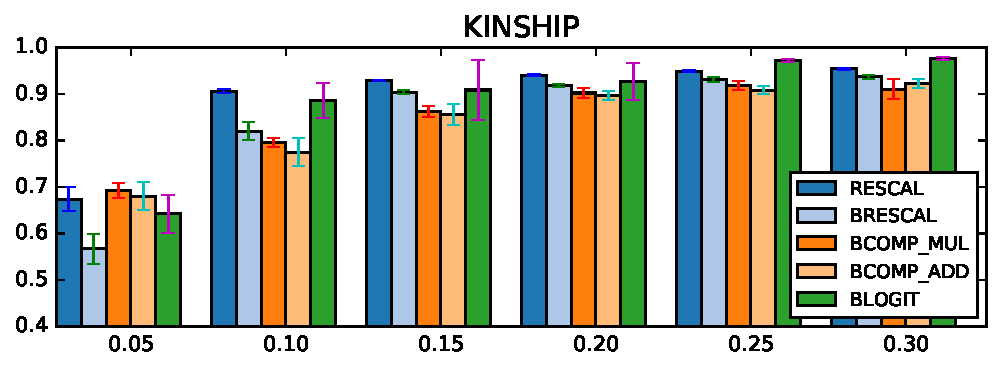
\includegraphics[width=\linewidth]{images/comp_training_error_kinship.pdf}
	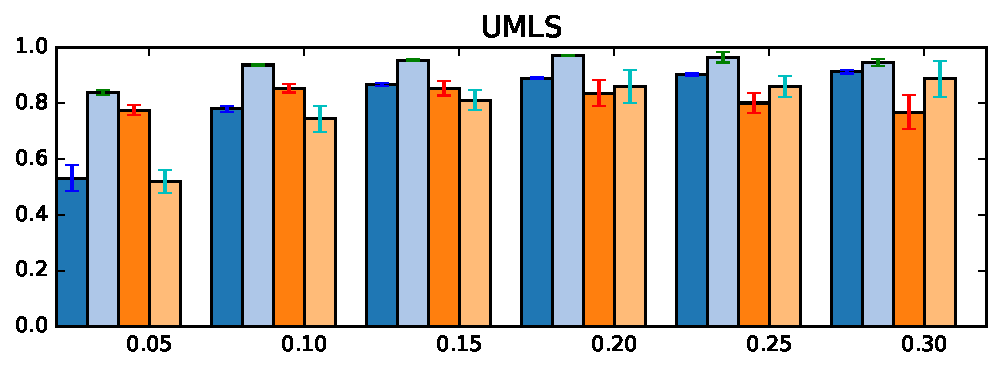
\includegraphics[width=\linewidth]{images/comp_training_error_umls.pdf}			
	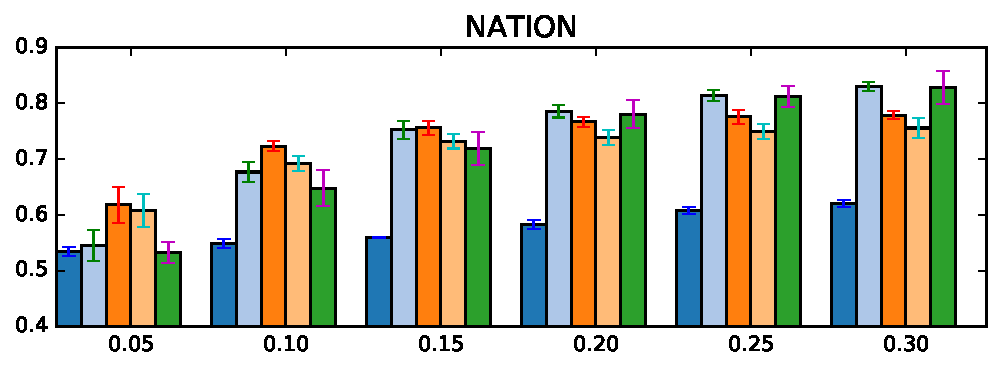
\includegraphics[width=\linewidth]{images/comp_training_error_nation.pdf}				
	\caption{\label{fig:r_vs_br} ROC-AUC scores of compositional models. The x-axis denotes the proportion of an observed triples including negative triples used for training models. We  use another 30\% of triples to evaluate the ROC-AUC score. In general, compositional models outperform BRESCAL and BLOGIT model when the size of training set is relatively small, whereas BRESCAL and BLOGIT perform slightly better than or comparable to the compositional models when the size of training set is relatively large. For UMLS dataset, the multiplicative compositional model consistently outperforms the other models across all training proportions.}
\end{figure}


From two triples:
$(i, k_1 ,j)$,  $(j, k_2, l)$

Compositional triple:
$(i, {c}(k_1, k_2), l)$

This compositional triple may have multiple path over the knowledge graph. For example, both pairs of triples $(i, k_1 ,j)$,  $(j, k_2, l)$ and $(i, k_1 ,m)$,  $(m, k_2, l)$ can be represented as $(i, {c}(k_1, k_2), l)$. To include the compositionality of the knowledge graph, we set  $x_{(i, {{c}(k_1, k_2)}, l)}$ be the number of path from entity $i$ to entity $j$ through relation $k_1$ and $k_2$.

We model a degree of the compositional relation as
\begin{align}
x_{(i, {{c}(k_1, k_2)}, l)} \sim \mathcal{N}(e_i^\top R_{{c}(k_1,k_2)} e_j, \sigma_{c}^2),
\end{align}
where $R_{{c}(k_1,k_2)} \in \mathbb{R}^{D\times D}$.

Let $\mathcal{C}^{L}$ be a set of all possible compositions of which length is up to length $L$, $c \in \mathcal{C}$ be a sequence of compositions, and $c(i)$ be $i$th index of a relation in sequence $c$. With the set of compositions $\mathcal{C}^{L}$, we can expand set of observed triples $\mathcal{X}^{t}$ to set of observed compositional triple $\mathcal{X}^{\mathcal{C}^{L}(t)}$ of which element $x_{icj}$ is a number of path from entity $i$ to entity $j$ through sequence of relations $c$ in $\mathcal{X}^{t}$.

\subsection{Additive Compositionality}
Let $R_{{c}} = \frac{1}{|c|}(R_{c(1)} + R_{c(2)} + \dots + R_{c(|c|)})$, then
\begin{align}
x_{(i, k_{{c}}, l)} \sim \mathcal{N}(e_i^\top R_c e_j, \sigma_{c}^2).
\end{align}

The conditional distribution of $e_i$ given $E_{-i}, \mathcal{R}, \mathcal{X}^{t}, \mathcal{X}^{L(t)}$ is 
\begin{align} \label{eqn:sample_e}
p(e_i |E_{-i}, \mathcal{R}, \mathcal{X}^{t}, \mathcal{X}^{L(t)}) &= \mathcal{N}(e_i | \mu_i, \Lambda_i^{-1}),
\end{align}
where
\begin{align*}
\mu_i &= \Lambda_i^{-1}\xi_i \\
\Lambda_i &= \frac{1}{\sigma_x^2} \sum_{jk : x_{ikj} \in \mathcal{X}^{t}} (R_k e_j)(R_k e_j)^\top \\
&\quad+ \frac{1}{\sigma_x^2} \sum_{jk : x_{jki} \in \mathcal{X}^{t}} (R_k^\top e_j)(R_k^\top e_j)^\top \\
&\quad + \frac{1}{\sigma_c^2} \sum_{jc : x_{icj} \in \mathcal{X}^{L(t)}} (R_c e_j)(R_c e_j)^\top \\
&\quad+ \frac{1}{\sigma_c^2} \sum_{jc : x_{jci} \in \mathcal{X}^{L(t)}} (R_c^\top e_j)(R_c^\top e_j)^\top + \frac{1}{\sigma_e^2} {I}_D \\
\xi_i &= \frac{1}{\sigma_x^2}\sum_{jk : x_{ikj} \in \mathcal{X}^{t}}  x_{ikj} R_{k} e_{j} + \frac{1}{\sigma_x^2}\sum_{jk : x_{jki} \in \mathcal{X}^{t}} x_{jki} R_{k}^\top e_{j} \\
& + \frac{1}{\sigma_c^2}\sum_{jc : x_{icj} \in \mathcal{X}^{L(t)}}  x_{icj} R_{c} e_{j} + \frac{1}{\sigma_c^2}\sum_{jc : x_{jci} \in \mathcal{X}^{L(t)}} x_{jci} R_{c}^\top e_{j}
\end{align*}

To compute the conditional distribution of $R_k$, we first decompose $R_c$ into two part where $R_c = \frac{1}{|c|} R_k + \frac{|c|-1}{|c|}R_{c/k}$, where $R_{c/k} = \sum_{k' \in c/k} R_{k'}$, if compositional sequence $c$ contains relation $k$. Vectorisation of $R_c$ and $R_{c/k}$ are represented as $r_c$ and $r_{c/k}$, respectively.

The degree of compositional path is represented with a decomposition as follows:
\begin{align}
x_{(i, c, l)} \sim \mathcal{N}(e_i^\top (\frac{1}{|c|} R_k + \frac{|c|-1}{|c|}R_{c/k}) e_j, \sigma_{c}^2).
\end{align}

Then, the conditional distribution $R_k$ given $R_{-k}, E, \mathcal{X}^{t}, \mathcal{X}^{L(t)}$ is
\begin{align}
\label{eqn:comp_cond_r}
p(R_k|E, \mathcal{X}^{t}, \mathcal{X}^{L(t)}, \sigma_r, \sigma_x)  &= \mathcal{N}(\text{vec}(R_k) | \mu_k, \Lambda_k^{-1}),
\end{align}
where
\begin{align*}
\mu_k &=\Lambda_k^{-1}\xi_k \\
\Lambda_k &= \frac{1}{\sigma_x^2} \sum_{ij:x_{ikj} \in \mathcal{X}^{t}} \bar{e}_{ij}\bar{e}_{ij}^\top + \frac{1}{\sigma_r^2} {I}_{D^2} \\
& +\frac{1}{|c|^2 \sigma_c^2} \sum_{ij:x_{icj} \in \mathcal{X}^{L(t)},\text{ }k \in c} \bar{e}_{ij} \bar{e}_{ij}^\top \\
\xi_k &=  \frac{1}{\sigma_x^2}\sum_{ij:x_{ikj} \in \mathcal{X}^{t}} x_{ikj} \bar{e}_{ij}\\
& +\frac{1}{|c| \sigma_c^2} \sum_{ij:x_{icj} \in \mathcal{X}^{L(t)},\text{ }k \in c} x_{icj} \bar{e}_{ij} - \frac{|c|-1}{|c|} \bar{e}_{ij} r_{c/k}^\top \bar{e}_{ij}\\
\bar{e}_{ij} &= e_{i} \otimes e_{j}.
\end{align*}

Note that the ordering of the relations in compositional sequence $c$ does not affect the value of compositional triple $(i, c, j)$.

\subsection{Multiplicative Compositionality}
Let compositional relation $R_c = R_{c(1)} R_{c(2)} \dots R_{c(|c|)}$.

If the determinant of latent relation $R_k$ is greater than 1, the compositional latent relation $R_c$ might be exploded after multiplying a long sequence of relations. To obtain a stable scale of compositional relation $R_c$, one may multiply decaying factor $\tau < 1$ after each composition. $R_c = \tau^{|c|-1} R_{c(1)} R_{c(2)} \dots R_{c(|c|)}$.

\begin{align}
x_{(i, c, j)} \sim \mathcal{N}(e_i^\top R_{c(1)}R_{c(2)} \dots R_{c(|c|-1)}R_{c(|c|)} e_j, \sigma_{c}^2)
\end{align}

If the compositional sequence $c$ contains relation $k$, the mean parameter of normal distribution contains $R_k$ in the middle of compositional sequence (i.e., $e_i^\top R_{c(1)}R_{c(2)} \dots R_{c(\delta_k)} \dots R_{c(|c|-1)}R_{c(|c|)} e_j$ where $\delta_k$ is the index of relation $k$). For notational simplicity, we will denote the left side $e_i^\top R_{c(1)}R_{c(2)} \dots R_{c(\delta_k -1)}$ as $\bar{e}_{ic(:\delta_k)}^\top$, and the right side $R_{c(\delta_k + 1)} \dots R_{c(|c|-1)}R_{c(|c|)} e_j$ as $\bar{e}_{ic(\delta_k:)}$, therefore we can rewrite the mean parameter as $\bar{e}_{ic(:\delta_k)}^\top R_{k} \bar{e}_{ic(\delta_k:)}$.

The conditional distribution of $e_i$ given the rest is the same as Equation $\ref{eqn:sample_e}$. The conditional of $R_k$ is
\begin{align}
p(R_k|E, \mathcal{X}, \sigma_r, \sigma_x)  &= \mathcal{N}(\text{vec}(R_k) | \mu_k, \Lambda_k^{-1}),
\end{align}
where
\begin{align*}
\mu_k &= \Lambda_k^{-1}\xi_k \\
\Lambda_k &= \frac{1}{\sigma_x^2} \sum_{ij:x_{ikj} \in \mathcal{X}^{t}} (e_i \otimes e_j)(e_i \otimes e_j)^\top + \frac{1}{\sigma_r^2} {I}_{D^2} \\
+ &\frac{1}{\sigma_c^2} \sum_{ij:x_{icj} \in \mathcal{X}^{L(t)}, \text{ }k \in c} (\bar{e}_{ic(:\delta_k)} \otimes \bar{e}_{jc(\delta_k:)})(\bar{e}_{ic(:\delta_k)} \otimes \bar{e}_{jc(\delta_k:)} )^\top \\
\xi_k &= \frac{1}{\sigma_x^2} \sum_{ij:x_{ikj} \in \mathcal{X}^{t}} x_{ikj} (e_{j} \otimes e_{i}) \\
& + \frac{1}{\sigma_c^2} \sum_{ij:x_{icj} \in \mathcal{X}^{L(t)}, \text{ }k\in c} x_{icj} (\bar{e}_{ic(:\delta_k)}  \otimes \bar{e}_{jc(\delta_k:)}).
\end{align*}


Thoughts: As the length of sequence $c$ increases, a small error in the first few multiplication will result a large differences in the final compositional relation. One way to mitigate this cascading error is to increase the variance of compositional triples as length of sequences increase.

\section{Experiments}
\subsection{Synthetic data}
\begin{figure}[t]
	\centering
	
	\subfigure[E=5, K=5, D=5\label{fig:syn1}]{
	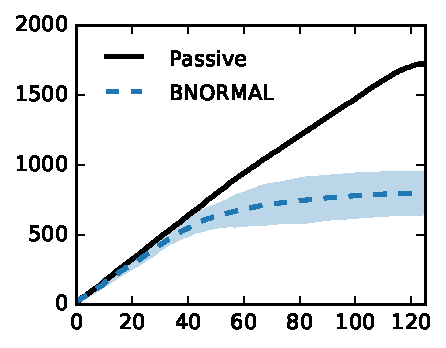
\includegraphics[width=0.42\linewidth]{images/toy_5_5_5.pdf}
	}
	\subfigure[E=10, K=10, D=5\label{fig:syn2}]{
	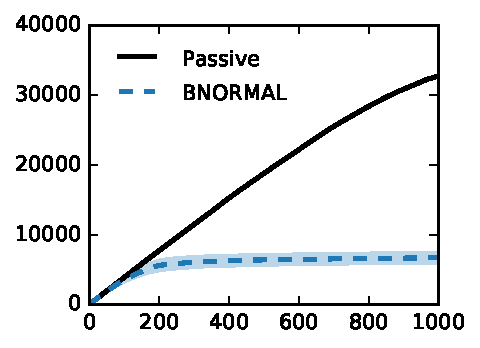
\includegraphics[width=0.45\linewidth]{images/toy_10_10_5.pdf}				
	}
%	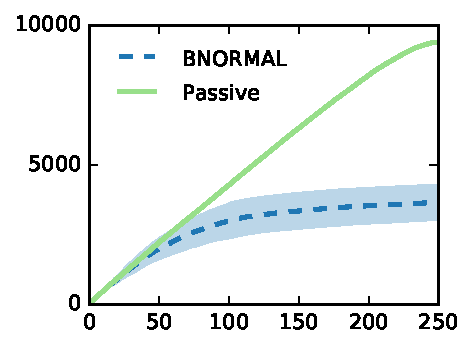
\includegraphics[width=0.32\linewidth]{images/toy_5_10_5.pdf}			
%	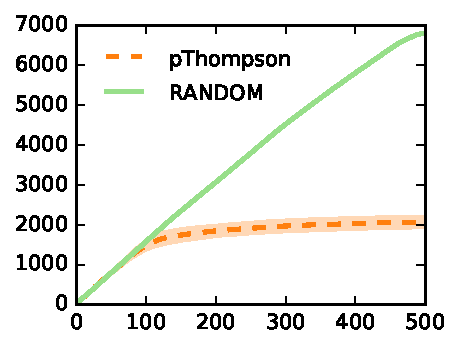
\includegraphics[width=0.32\linewidth]{images/toy_10_5_5.pdf}				
	\caption{\label{fig:synthetic} Cumulative regret of particle Thompson sampling on different sizes of the synthetic dataset. The synthetic dataset is generated by the model assumption (Eq. \ref{eqn:entity_gen} - \ref{eqn:triple_gen}). We compared the particle Thompson sampling with random sampling method. The averaged cumulative regrets are plotted with one standard error. As the model obtained more and more labeled samples from Thompson sampling, the cumulative regrets are converged. This result  indicates the particle sampling correctly inferred latent features of entities and relations on the synthetic datasets. // The results are averaged over 10 runs. $\sigma_e = 10$, $\sigma_r=10$, $\sigma_x=0.1$, $H=5$.}
\end{figure}

\subsection{Synthetic data}
\begin{figure}[t]
	\centering
	
	\subfigure[KINSHIP]{
	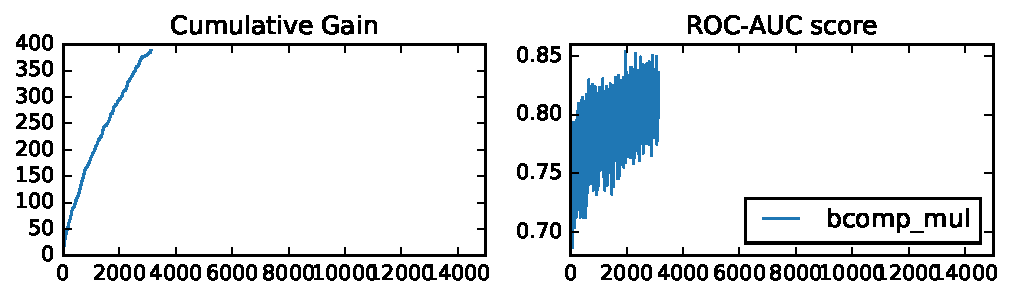
\includegraphics[width=\linewidth]{images/cum_gain_roc_umls.pdf}
	}
	\subfigure[UMLS]{
	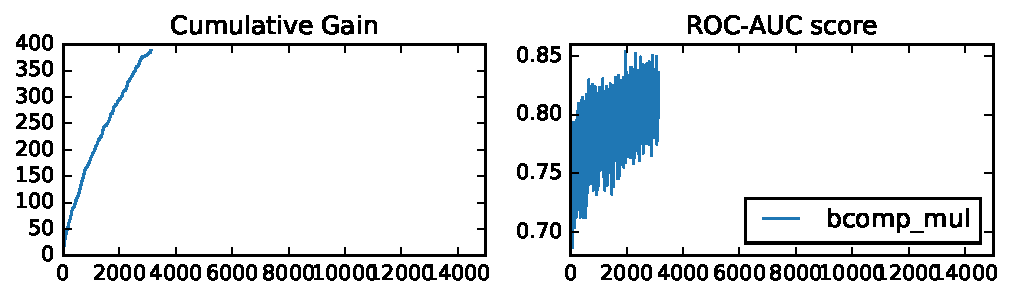
\includegraphics[width=\linewidth]{images/cum_gain_roc_umls.pdf}				
	}
	\subfigure[NATION]{
	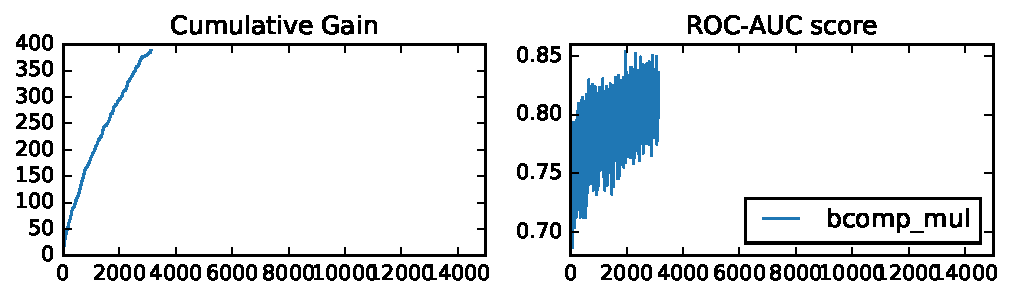
\includegraphics[width=\linewidth]{images/cum_gain_roc_umls.pdf}				
	}	
	\caption{Placeholder for the future results. Will include the cumulative gain and ROC-AUC score of the developed models with the active and passive learning methods. We will see how the compositional model performs to compare with other models without any initial observation (May include the IBM model without any initial observation).}
\end{figure}

\section{Unstructured thoughts}

\begin{description}
  \item[Not useful theorem] In \cite{kawale2015efficient}, the theorem does not really give
  a setting that is used in the paper.
  \item[Logistic regression] For outputs which are binary, instead of a Gaussian assumption on
  $x$, we can use logistic regression. See
   \url{http://people.csail.mit.edu/romer/papers/TISTRespPredAds.pdf}
  \item[Choosing triples] For entity $e_i$ related via relation $R_k$ to entity $e_j$, we want
  an active learning algorithm that will choose triples $e_i R_k e_j$ that corresponds to
  $x_{ikj}$. This will not have a bandit regret bound, since we only choose each triple once.
  \item[Contextual Bandits] There are two groups of three possible assumptions for contextual
  bandits:
  \begin{enumerate}
    \item Two elements of the tuple as context, choose only one element
    \begin{itemize}
      \item $e_iR_k$ context, $e_j$ arms
      \item $e_i, e_j$ context, $R_k$ arms
      \item $R_ke_j$ context, $e_i$ arms
    \end{itemize}
    \item One element of the tuple as context, choose two elements
    \begin{itemize}
      \item $e_i$ context, $R_k e_j$ arms
      \item $R_k$ context, $e_i, e_j$ arms
      \item $e_j$ context, $e_iR_k$ arms
    \end{itemize}
  \end{enumerate}
\end{description}

\begin{table}
\centering
\caption{\label{tbl:dataset}Description of datasets.}
\begin{tabular}{l | r | r | r | r}
Dataset &  \# rel & \# entities & \# triples & sparsity \\ \hline
Kinship & 26 & 104  & 10,790 & 0.038 \\
UMLS & 49 &135  & 6,752 & 0.008 \\
Nation & 56 & 14  & 2,024 & 0.184 \\
%Wordnet & 11 & 38,696  &123,429 & 7.5e-06\\
%Wordnet(N) & 10 & 836 & 1,766 & 2.5e-04\\
\end{tabular}
\end{table}

% In the unusual situation where you want a paper to appear in the
% references without citing it in the main text, use \nocite

\bibliography{icml2016}
\bibliographystyle{icml2016}

\section*{Appendix}
\subsection*{Detailed derivation of Equation \ref{eqn:comp_cond_r}}

\begin{align*}
&p(R_k | E, R_{-k}, \mathcal{X}) \propto p(\mathcal{X} | R, E)p(R_k)&\\
&\propto \prod_{x_{ikj}}\exp\bigg\{-\frac{(x_{ikj} - e_i^\top R_k e_j)^2}{2\sigma_x^2}\bigg\} &\\
& \quad\prod_{x_{icj}} \exp\bigg\{-\frac{(x_{icj} - e_i^\top R_c e_j)^2}{2\sigma_c^2}\bigg\} \exp\bigg\{-\frac{r_k^\top r_k}{2\sigma_r^2}\bigg\}&\\
&= \exp\bigg\{-\frac{\sum_{x_{ikj}}(x_{ikj} - \bar{e}_{ij}^\top r_k)^2}{2\sigma_x^2} &\\
&\quad- \frac{\sum_{x_{icj}}(x_{icj} - \bar{e}_{ij}^\top r_c)^2}{2\sigma_c^2} -\frac{r_k^\top r_k}{2\sigma_r^2} \bigg\}&\\
&= \exp\bigg\{-\frac{\sum_{x_{ikj}}(x_{ikj} - \bar{e}_{ij}^\top r_k)^2}{2\sigma_x^2} &\\ 
&\quad-\frac{\sum_{x_{icj}}(x_{icj} - \bar{e}_{ij}^\top (\frac{1}{|c|}r_k + \frac{|c|-1}{|c|})r_{c/k})^2}{2\sigma_c^2} -\frac{r_k^\top r_k}{2\sigma_r^2} \bigg\}&\\
&= \exp\bigg\{ -\frac{\sum_{x_{ikj}}- 2 x_{ikj} \bar{e}_{ij}^\top r_k + r_k^\top \bar{e}_{ij} \bar{e}_{ij}^\top r_k }{2\sigma_x^2} &\\
&\quad-\frac{\sum_{x_{icj}} \frac{2}{|c|} r_k ^\top (x_{icj} - \frac{(|c|-1)}{|c|} \bar{e}_{ij}^\top r_{c/k}) + (\frac{1}{|c|^2}r_k^\top \bar{e}_{ij} \bar{e}_{ij}^\top r_k)}{2\sigma_c^2} &\\
&\quad-\frac{r_k^\top r_k}{2\sigma_r^2} + const \bigg\}&\\
&\propto \exp\bigg\{ - \frac{1}{2}r_k^\top(\frac{1}{\sigma_x^2}\sum_{x_{ikj}} \bar{e}_{ij}\bar{e}_{ij}^\top + \frac{1}{|c|^2\sigma_c^2}\sum_{x_{icj}} \bar{e}_{ij}\bar{e}_{ij}^\top + \frac{1}{\sigma_r^2}I) r_k  &\\
&- r_k^\top \Big(\frac{\sum_{x_{ikj}}-x_{ikj}\bar{e}_{ij}}{\sigma_x^2} + \frac{\sum_{x_{icj}} |c|^{-1} (x_{icj} - \frac{(|c|-1)}{|c|} \bar{e}_{ij}^\top r_{c/k})}{\sigma_c^2} \Big)&
\end{align*}
Completing the square results Equation \ref{eqn:comp_cond_r}.


\end{document}


% This document was modified from the file originally made available by
% Pat Langley and Andrea Danyluk for ICML-2K. This version was
% created by Lise Getoor and Tobias Scheffer, it was slightly modified
% from the 2010 version by Thorsten Joachims & Johannes Fuernkranz,
% slightly modified from the 2009 version by Kiri Wagstaff and
% Sam Roweis's 2008 version, which is slightly modified from
% Prasad Tadepalli's 2007 version which is a lightly
% changed version of the previous year's version by Andrew Moore,
% which was in turn edited from those of Kristian Kersting and
% Codrina Lauth. Alex Smola contributed to the algorithmic style files.
